\section{Estimación por intervalor}
\subsection{Introducción}
\begin{tcolorbox}[colback=blue!5!white, colframe=blue!75!black, title=\textbf{Estimación paramétrica}]
En el contecto e la estimación paramétrica, queremos aprovechar nuestro conocimiento sobre la distribución muestral de estimador, para proporcionar margen de error y riesgo.
\end{tcolorbox}
\begin{tcolorbox}[colback=blue!5!white, colframe=blue!75!black, title=\textbf{Bootstrap}]
También construiremos intervalos de confianza basados en percentiles Bootstrap.
\end{tcolorbox}
\begin{tcolorbox}[colback=red!5!white, colframe=red!75!black, title=\textbf{Idea básica}]
Supongamos:
\begin{itemize}[label=\textbullet]
    \item $X\sim \mathcal{N}(\mu,4)$.
    \item Consideramos una muestra aleatoria simple $X_1,\dots,X_4$, estimamos $\mu$ con $\overline{X}$.
\end{itemize}
Deducimos:
\begin{itemize}[label=\textbullet]
    \item Sabemos que $\overline{X}\sim \mathcal{N}(\mu,1)$.
    \item Implica: el 95\% de los valores de $\overline{X}$ está aproximadamente entre $\mu\pm 2$.
    \item Si sé dónde está $\mu$, sé que, con probabilidad 0.95, $\overline{X}$ se encuentre a menos de 2 unidades.
    \item Ahora al revés: si he observado un valor de $\overline{X}$, ¿dónde está $\mu$? la probabilidad de que $\mu$ se encuentre a menos de 2 unidades de $\overline{X}$ es 0.95.
\end{itemize}
\end{tcolorbox}
La probabilidad de que, habiendo observado un valor de $\overline{X},\mu$ se encuentre a menos de 2 unidades es $0.95$.
 \[
\mu\in \overline{X}\pm 2,\quad \text{con probabilidad 0.95}
\] 
\begin{itemize}[label=\textbullet]
    \item $\overline{X}\pm 2$ es un intervalo aleatorio.
    \item Para una muestra concreta que extraigamos, será $\overline{x}\pm 2$.
    \item $\pm 2$ expresa el margen de error.
    \item "con probabilidad 0.95" expresa la confianza que tenemos en que nuestra información sea cierta.
    \item Corremos un riesgo de error de 0.05 al afirmar,  $\mu\in \overline{X}\pm 2$.
\end{itemize}
\begin{tcolorbox}[colback=blue!5!white, colframe=blue!75!black, title=\textbf{Definición}]
\begin{itemize}[label=\textbullet]
    \item $(X_1,\dots,X_n)$ una muestra asociada a $f_\theta$.
    \item Un \lb{intervalo de estimación} está asociado por dos estadísticos $I(X_1,\dots,X_n)$ (extremo inferior) y $D(X_1,\dots,X_n)$ (extremos superior) y persigue capturar el valor del parámetro $\theta$.
\end{itemize}
\end{tcolorbox}
\begin{tcolorbox}[colback=red!5!white, colframe=red!75!black, title=\textbf{Un intervalo de estimación es aleatorio}]
\begin{itemize}[label=\textbullet]
    \item Sus extremos dependen de la muestra concreta escogida.
    \item $\theta \in [I(X_1,\dots,X_n),D(X_1,\dots,X_n)]$ define un suceso aleatorio.
    \item La probabilidad de este suceso $\mathbb{P}_\theta[\theta\in [I(X_1,\dots,X_n),D(X_1,\dots,X_n)]]$ se llama \textbf{nivel de cobertura} del intervalo para este valor de $\theta$.
    \item El nivel de cobertura depende de $\theta$.
\end{itemize}
\end{tcolorbox}
\subsection{Nivel de confianza}
\begin{itemize}[label=\color{red}\textbullet, leftmargin=*]
    \item \lb{Nivel de cobertura} \[
            \theta\longmapsto \mathbb{P}_\theta[\theta\in [I(X_1,\dots,X_n),D(X_1,\dots,X_n)]]]
    \] 
    El \lb{nivel de confianza} es el valor mínimo del nivel de cobertura calculado cuando varía $\theta$. 
\end{itemize}
\begin{tcolorbox}[colback=olive!5!white, colframe=olive!75!black, title=\textbf{Confianza vs Precisión}]
Deberemos buscar una alta confianza pero sin sacrificar en exceso la precisión.
\end{tcolorbox}
\subsection{Un procedimiento general de construcción}
Se aplica en muchas situaciones de modelización.
\begin{tcolorbox}[colback=blue!5!white, colframe=blue!75!black, title=\textbf{Procedimiento}]
\begin{itemize}[label=\textbullet]
    \item Nos fijamos el "nivel de riesgo", $0<\alpha<1$, por ejemplo, $0.1,0.05$, o  $0.01$.
    \item Buscamos  $T(X_1,\dots,X_n)$ que se \lb{pivotal}, es decir, que su distribución no depende de $\theta$.
    \item Escogemos dos cotas $a$ y  $b$:  \[
            \mathbb{P}_\theta[a\le T(X_1,\dots,X_n)\le b]=1-\alpha,\quad \forall \theta\in \Theta.
    \] 
\item Procuramos despejar $\theta$: \[
        \mathbb{P}_\theta[I(X_1,\dots,X_n)\le \theta\le D(X_1,\dots,X_n)]=1-\alpha.
\] 
\end{itemize}
\end{tcolorbox}
\begin{tcolorbox}[colback=red!5!white, colframe=red!75!black, title=\textbf{Nota}]
\begin{itemize}[label=\textbullet]
    \item $T$ es pivotal $\longrightarrow $ el nivel de cobertura $1-\alpha$ de $[I(X_1,\dots,X_n),D(X_1,\dots,X_n)]$ no depende de $\theta$.
    \item $1-\alpha$ es el nivel de confianza.
\end{itemize}
\end{tcolorbox}
\subsection{Intervalo de confianza para la media $\mu$ de $X\sim \mathcal{N}(\mu,\sigma^2),\sigma$ conocida}

\lb{Consideramos una muestra aleatoria simple de una distribución $X\sim \mathcal{N}(\mu,\sigma^2)$. El valor de $\sigma^2$ es conocido}
\begin{itemize}[label=\textbullet]
    \item Usaremos $\overline{X}$ para estimar $\mu$.
\end{itemize}
Estadístico pivotal: \[
    T(X_1,\dots,X_n;\theta)=\dfrac{\overline{X}-\mu}{\sigma / \sqrt{n} }\sim \mathcal{N}(0,1).
\] 
\begin{itemize}[label=\textbullet]
    \item Dibujamos en la densidad del estadístico pivotal $\dfrac{\overline{X}-\mu}{\sigma / \sqrt{n} }$, una región central que represente el $100(1-\alpha)\%$ del área total.
\end{itemize}
\begin{center}
    \includegraphics[width=0.5\textwidth]{"Tema 3/figures/Figure 1"}
\end{center}
\begin{tcolorbox}[colback=olive!5!white, colframe=olive!75!black, title=\textbf{Cuantil}]
Para $0\le u\le 1, z_u$ es el \textbf{cuantil} $u$ de una $\mathcal{N}(0,1)$, es decir, el valor que cumple $\mathbb{P}(Z\le z_u)=u$.
\end{tcolorbox}
\[
\mathbb{P}\left[ -z_{1-\alpha /2}\le \dfrac{\overline{X}-\mu}{\sigma / \sqrt{n} }\le z_{1-\alpha /2} \right] =1-\alpha.
\] 
Despejamos $\mu$:
\begin{itemize}[label=\textbullet]
    \item $\mathbb{P}\left[ \overline{X}-z_{1-\alpha / 2}\dfrac{\sigma}{\sqrt{n} }\le \mu\le \overline{X}+z_{1-\alpha /2}\dfrac{\sigma}{\sqrt{n} } \right] =1-\alpha$
    \item El \lb{intervalo de confianza} al $100(1-\alpha)\%$ para $\mu$ es: \[
    \mu\in \left( \overline{X}-z_{1-\alpha / 2}\dfrac{\sigma}{\sqrt{n} };\overline{X}+z_{1-\alpha / 2}\dfrac{\sigma}{\sqrt{n} } \right) .
    \] 
\item De forma equivalente: $\mu\in \overline{X}\pm z_{1-\alpha / 2}\dfrac{\sigma}{\sqrt{n} }.$
\end{itemize}
\begin{tcolorbox}[colback=olive!5!white, colframe=olive!75!black, title=\textbf{Margen de error}]
$z_{1-\alpha /2}\dfrac{\sigma}{\sqrt{n} }$ se llama \textbf{término de error}. 
\end{tcolorbox}
\subsubsection{Interpretación}
\begin{tcolorbox}[colback=red!5!white, colframe=red!75!black, title=\textbf{Importante}]
\begin{itemize}[label=\textbullet]
    \item El intervalo de confianza $\left[ \overline{X}-z_{1-\alpha /2}\dfrac{\sigma}{\sqrt{n} };\overline{X}+z_{1-\alpha /2}\dfrac{\sigma}{\sqrt{n} } \right] $ es un intervalo \textbf{aleatorio}.
    \item Al extraer una muestra, tengo una probabilidad $\alpha$ de que, al afirmar que $\mu$ se encuentra en $\left[ \overline{X}-z_{1-\alpha / 2}\dfrac{\sigma}{\sqrt{n} };\overline{X}-z_{1-\alpha /2}\dfrac{\sigma}{\sqrt{n} } \right] $, me equivoque.
\end{itemize}
\end{tcolorbox}
\begin{center}
    \includegraphics[width=0.7\textwidth]{"Tema 3/figures/Figure 2"}
\end{center}

\lb{\underline{Ejemplo:} } 

\begin{itemize}[label=\textbullet]
    \item Queremos estimar la longitud media de un artículo producido por una máquina.
    \item Por experiencia, sabemos que es razonable modelizar la distribución de los valores de la longitud de los artículos producidos por una distribución Normal con media $\mu$ y desviación típica a 0.05.
    \item Para estimar $\mu$ extraemos una muestra de 5 artículos: \[
    20.1,20.05,19.95,19.99.
    \]
\item Construir un intervalo de confianza al 90\%.
\end{itemize}
\begin{minipage}{0.45\textwidth}
    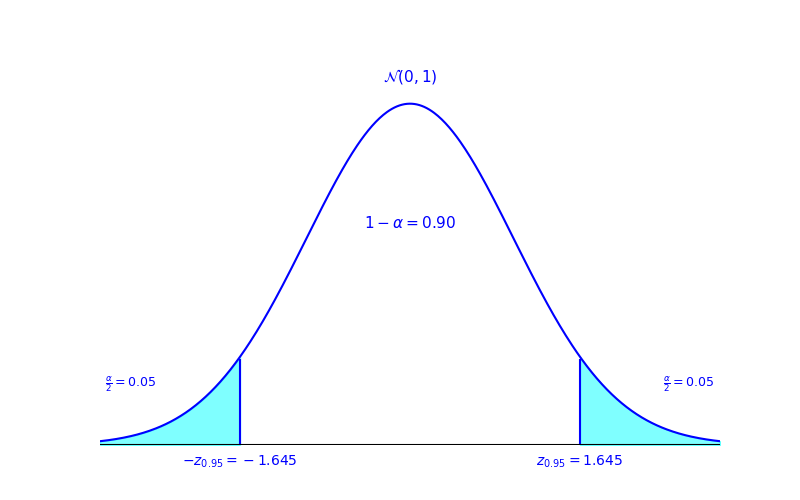
\includegraphics[width=\linewidth]{Tema 3/figures/Figure 3}
\end{minipage}
$\begin{array}{l}
    \overline{x}=20.02\\
1-\alpha=0.09\\
\alpha=0.1\\
\dfrac{\alpha}{2}=0.05\\
\left(20.2\mp 1.645 \dfrac{0.05}{\sqrt{5} }\right)=(20.02\mp 0.0367) = (19.9833, 20.0588)
\end{array}$

\subsection{Comentarios importantes}
\begin{tcolorbox}[colback=olive!5!white, colframe=olive!75!black, title=\textbf{Si $X$ no es Normal}]
\begin{itemize}[label=\textbullet]
    \item Hemos trabajado con la hipótesis de que $X$ es Normal para encontrar el estadístico pivotal $\dfrac{\overline{X}-\mu}{\sigma / \sqrt{n} }\sim \mathcal{N}(0,1)$.
    \item Si $X$ no es Normal, no podemos garantizar la confianza especificada.
    \item Sin embargo, si $n$ grande, tenemos por el Teorema Central del Límite \[
    \dfrac{\overline{X}-\mu}{\sigma / \sqrt{n} }\sim \mathcal{N}(0,1),\text{ aproximiadamente, }
    \] 
    entonces la confianza especificada no será exacta pero casi\dots
\end{itemize}
\end{tcolorbox}
\subsubsection{Factores que afectan a la precisión de la estimación}
\begin{tcolorbox}[colback=olive!5!white, colframe=olive!75!black, title=\textbf{El margen de error es $z_{1-\alpha /2}\dfrac{\sigma}{\sqrt{n} }$.}]
\begin{itemize}[label=\textbullet]
    \item $n\uparrow\longrightarrow \text{ precisión }\uparrow$
    \item $\sigma\uparrow\longrightarrow \text{ precisión }\downarrow$ 
    \item Confianza $\uparrow\longrightarrow $ precisión $\downarrow$
\end{itemize}
\end{tcolorbox}
\subsubsection{Determinación del tamaño muestral}
\begin{tcolorbox}[colback=blue!5!white, colframe=blue!75!black, title=\textbf{Contexto}]
Antes de extraer la muestra:
\begin{itemize}[label=\textbullet]
    \item Tenemos decidido el valor de $\sigma$.
    \item Tenemos decidido la confianza con la que trabajamos.
    \item Tenemos decidio el margen de error máximo $max$ que estamos dispuestos a comenter.
\end{itemize}
¿Qué tamaño de la muestra debemos escoger?
\end{tcolorbox}
Margen de error: $z_{1-\alpha /2}\dfrac{\sigma}{\sqrt{n} }\le max.\longrightarrow $ Despejamos $n$
\subsubsection{Otros modelos, estadísticos pivotales}
 \begin{tcolorbox}[colback=blue!5!white, colframe=blue!75!black, title=\textbf{$X\sim \mathcal{N}(\mu,\sigma^2)$, estimamos $\mu,\sigma$ desconocida}]
Estadístico pivotal: \[
T=\dfrac{\overline{X}-\mu}{S / \sqrt{n} }\sim t_{n-1}
\] 
\end{tcolorbox}

Debemos encontrar valores $a$ y $b$ tales que:

\begin{minipage}{0.45\textwidth}
    \includegraphics[width=\linewidth]{"Tema 3/figures/Figure 4"}
\end{minipage}$\begin{array}{l}
    P\left[ a\le \dfrac{\overline{X}-\mu}{S / \sqrt{n} }\le b \right] \\
    P\left[ -t_{n-1,1-\frac{\alpha}{2}}\le \dfrac{\overline{X}-\mu}{S / \sqrt{n} }\le t_{n-1,1-\frac{\alpha}{2} } \right] \\
    P\left[ X-t_{n-1,1-\frac{\alpha}{2} }\dfrac{S}{\sqrt{n} }\le \dfrac{\overline{X}-\mu}{S / \sqrt{n} }\le X+t_{n-1,1-\frac{\alpha}{2} }\dfrac{S}{\sqrt{n} } \right] =1-\alpha
\end{array}$

Obteniendo como I.C aleatorio a nivel $100(1-\alpha)\%$ \[
X-t_{n-1,1-\frac{\alpha}{2} }\dfrac{S}{\sqrt{n} }
\] 
\begin{tcolorbox}[colback=blue!5!white, colframe=blue!75!black, title=\textbf{$X\sim \mathcal{N}(\mu,\sigma^2)$, estimamos $\sigma^2$}]
Estadístico pivotal: \[
\dfrac{(n-1)S_n^2}{\sigma^2}\sim \chi_{n-1}^2
\] 
\end{tcolorbox}
I.C para $\sigma^2$ al nivel de confianza $(1-\alpha)100\%$ \[
T=\dfrac{(n-1)s^2}{\sigma^2}\leadsto \chi_{n-1}^2
\] 
Debemos encontrar valores $a$ y $b$ tales que: $P\left[ a\le \dfrac{(n-1)s^2}{\sigma^2}\le b \right]=1-\alpha $

\begin{minipage}{0.45\textwidth}
    \includegraphics[width=\linewidth]{"Tema 3/figures/Figure 5"}
\end{minipage}
$\begin{array}{l}
    P\left[ -\chi_{n-1,\frac{1-\alpha}{2} }^2\le \dfrac{(n-1)s^2}{\sigma^2}\le \chi_{n-1,1-\frac{\alpha}{2} }^2 \right] =1-\alpha\\
    P\left[ -\dfrac{1}{\chi_{n-1,1-\frac{\alpha}{2}}} \le  \dfrac{\sigma^2}{(n-1)s^2}\le \dfrac{1}{\chi_{n-1,1-\frac{\alpha}{2} }^2} \right] =1-\alpha\\
    P\left[ -\dfrac{(n-1)s^2}{\chi_{n-1,1-\frac{\alpha}{2} }^2}\le \sigma^2\le \dfrac{(n-1)s^2}{\chi_{n-1,1-\frac{\alpha}{2} }^2} \right] =1-\alpha
\end{array}$
\begin{tcolorbox}[colback=blue!5!white, colframe=blue!75!black, title=\textbf{$X\sim \mathrm{Bernoulli}$, estimamos $p$}]
Estadístico pivotal aproximado: \[
    \dfrac{\hat{p}-p}{\sqrt{\hat{p}(1-\hat{p}) / n} }\sim \mathcal{N}(0,1)\quad \mathrm{aprox}.
\] 
\end{tcolorbox}
\begin{tcolorbox}[colback=blue!5!white, colframe=blue!75!black, title=\textbf{Diferencias de dos variables aleatorias normales}]
Contexto:
\begin{itemize}[label=\textbullet]
\item $X\sim \mathcal{N}(\mu_X,\sigma_X^2)$ y $Y\sim \mathcal{N}(\mu_Y,\sigma_Y^2)$, independientes.
\item Dos muestras aleatorias simples $X_1,\dots,X_{n_X}$, de $X$ e  $Y_1,\dots,Y_{n_Y}$, de $Y$.
\item Suponemos que conocemos $\sigma_{X}^2$ y $\sigma_Y^2$.
\end{itemize}
Estadístico pivotal: \[
\dfrac{\overline{X}-\overline{Y}-(\mu_X-\mu_Y)}{\sqrt{\dfrac{\sigma_X^2}{n_X}+ \dfrac{\sigma_Y^2}{n_Y}} }\sim \mathcal{N}(0,1).
\] 
\end{tcolorbox}
\begin{tcolorbox}[colback=blue!5!white, colframe=blue!75!black, title=\textbf{Diferencias de dos variables aleatorias normales}]
Contexto:
\begin{itemize}[label=\textbullet]
\item $X\sim \mathcal{N}(\mu_X,\sigma_X^2)$ y $Y\sim \mathcal{N}(\mu_Y,\sigma_Y^2)$, independientes.
\item Dos muestras aleatorias simples $X_1,\dots,X_{n_X}$, de $X$ e  $Y_1,\dots,Y_{n_Y}$, de $Y$.
\item Desconocemos $\sigma_X^2$ y $\sigma_Y^2$, pero las suponemos iguales, $\sigma_X^2=\sigma_Y^2$.
\end{itemize}
Estadístico pivotal: \[
    \dfrac{\overline{X}-\overline{Y}-(\mu_X-\mu_Y)}{\sqrt{\frac{(n_{X}-1)S_X^2+(n_y-1)S_Y^2}{n_X+n_Y-2} }\sqrt{\frac{1}{n_X} +\frac{1}{n_Y} }  }\sim  t_{n_X+n_Y-2}.
\] 
\end{tcolorbox}
\begin{tcolorbox}[colback=blue!5!white, colframe=blue!75!black, title=\textbf{Cociente de varianzas, para dos variables aleatorias normales}]
Contexto: 
\begin{itemize}[label=\textbullet]
    \item $X\sim \mathcal{N}(\mu_X,\sigma_X^2)$ y $Y\sim \mathcal{N}(\mu_Y,\sigma_Y^2)$, independientes.
\item Dos muestras aleatorias simples $X_1,\dots,X_{n_X}$, de $X$ e  $Y_1,\dots,Y_{n_Y}$, de $Y$.
\end{itemize}
Estadístico pivotal: \[
\dfrac{S_X^2 / \sigma_X^2}{S_Y^2 / \sigma_Y^2}\sim F_{n_X-1,n_Y-1}.
\] 
\end{tcolorbox}
\begin{minipage}{0.45\textwidth}
    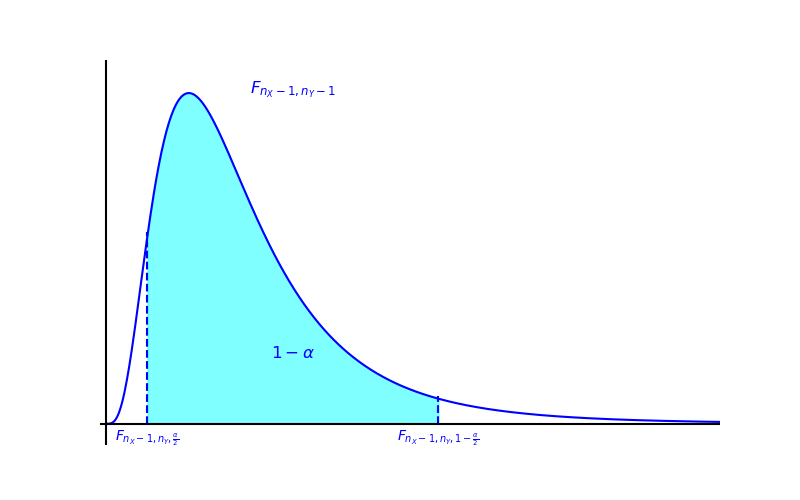
\includegraphics[width=\textwidth]{Tema 3/figures/Figure 6}
\end{minipage}$\begin{array}{l}
    P\left[ a\le \dfrac{S_X^2 / \sigma_X^2}{S_Y^2 / \sigma_Y^2}\le b \right] =1-\alpha\\
    P\left[ F_{n_X-1,n_Y-1,\frac{\alpha}{2} }\le \dfrac{S_X^2 / \sigma_X^2}{S_Y^2 / \sigma_Y^2}\le F_{n_X-1,n_Y-1,1-\frac{\alpha}{2} } \right] 
\end{array}$ 

\[
\bboxed{P\left[ \dfrac{S_Y^2}{S_X^2}F_{n_X-1,n_Y-1,\frac{\alpha}{2} }\le \dfrac{\sigma_Y^2}{\sigma_X^2}F_{n_X-1,n_Y-1,1-\frac{\alpha}{2} } \right] =1-\alpha}
\]
\subsection{Intervalos de confianza basados en el Bootstrap}
\begin{tcolorbox}[colback=blue!5!white, colframe=blue!75!black, title=\textbf{Una primera aproximación}]
\begin{itemize}[label=\textbullet]
    \item Podemos usar los cuantiles de una distribución normal, al igua que lo hacemos para construir un IC para la media de una normal.
    \item Se suele usar la aproximación si $n$ es grande: $\dfrac{\hat{\theta}_n-\theta}{\hat{se}}\sim \mathcal{N}(0,1)$.
    \item Por ejemplo al 95\%: $\hat{\theta}_n+1.96\cdot \hat{se}$, o aproximadamente $\hat{\theta}_n+2\cdot \hat{se}$.
\end{itemize}
\end{tcolorbox}
\begin{lstlisting}
ingresos <- c(22010, 43950, 31416, 143200, 19298, 21521, 60025, 24320, 18221, 29528) 
\end{lstlisting}
\begin{lstlisting}
library(tidyverse)
B <- 200
lista_boot_muestras <- replicate(
      B,
      sample(ingresos, size = length(ingresos), replace = TRUE),
      simplify = FALSE
)
valores_medianas <- map_dbl(lista_boot_muestras, median)
error_estandar_estimacion <- sd(valores_medianas)
\end{lstlisting}
En el ejemplo de los ingresos, obtenemos para la mediana: $26924\pm 12311$.
\begin{tcolorbox}[colback=olive!5!white, colframe=olive!75!black, title=\textbf{La construcción anterior es una aproximación}]
\begin{itemize}[label=\textbullet]
    \item Es posible, en particular si $n$ no es grande o si la distribución es asimétrica, que el nivel de confianza no sea correcto.
    \item Siempre produce intervalos simétricos, lo que puede ser una limitación.
    \item Para mejorar la veracidad del intervalo construido, vamos a ver el intervalo de confianza basado en percentiles Bootstrap.
\end{itemize}
\end{tcolorbox}
\begin{tcolorbox}[colback=blue!5!white, colframe=blue!75!black, title=\textbf{Procedimiento}]
\begin{itemize}[label=\textbullet]
    \item Habiendo observado una muestra $\mathbf{x}$, queremos estimar $\theta$, usando un estimador $\hat{\theta}=T(\mathbf{x})$.
    \item Simulamos un gran número $B$ de muestras Bootstrap a partir de $\mathbf{x}$, obteniendo $\mathbf{x}^{*1},\dots,\mathbf{x}^{*n}$.
    \item Calculamos para cada muestra Bootstrap, $\hat{\theta}^{*b}=T(\mathbf{x}^{*b})$.
    \item Si $1-\alpha$ es el nivel de confianza, consideramos el conjunto $\hat{\theta}^{*1},\dots,\hat{\theta}^{*B}$ y calculamos:
        \begin{itemize}[label=\textrightarrow]
            \item $\hat{\theta}^{*(\alpha /2)}$ el percentil $100\cdot \dfrac{\alpha}{2}$.
            \item $\hat{\theta}^{*(1-\alpha /2)}$ el percentil $100\cdot \left(1-\dfrac{\alpha}{2}\right)$.
        \end{itemize}
    \item Nuestro intervalo al $100(1-\alpha)$ es $[\hat{\theta}^{*(\alpha /2)},\hat{\theta}^{*(1-\alpha /2)}]$.
\end{itemize}
\end{tcolorbox}
\begin{tcolorbox}[colback=olive!5!white, colframe=olive!75!black, title=\textbf{¿Cómo se calcula el percentil $100\cdot p$?}]
    Si tenemos un conjunto $\hat{\theta}^{*1},\dots,\hat{\theta}^{*B}, B$ grande, para calcular el percentil $100\cdot p$ para $0\le p\le 1$, podemos seguir estos pasos:
    \begin{itemize}[label=\textbullet]
        \item Ordenamos los datos de menor a mayor.
        \item Calculamos un índice como $i=p\times (B+1)$, donde $B$ es el número de observaciones.
        \item Si  $i$ es un número entero, podemos interpolar entre los puntos de datos adyacentes.
            \begin{itemize}[label=\textbullet]
                \item Existen distintas posibilidades para la interpolación.
                \item En \lb{\textbf{\texttt{R}}}: Usamos la función \lb{\textbf{\texttt{quantile}}}, que admite hasta 9 tipos de interpolación con el argumento \lb{\textbf{\texttt{type}}}.
            \end{itemize}
    \end{itemize}
\end{tcolorbox}
\subsubsection{Aplicación con el ejemplo de los ingresos}
Simulamos $B=10000$ muestras Bootstrap, calculamos las 10000 medianas $\hat{\theta}^{*1},\dots,\hat{\theta}^{*10000}$ y hacemos un histograma:
\begin{center}
    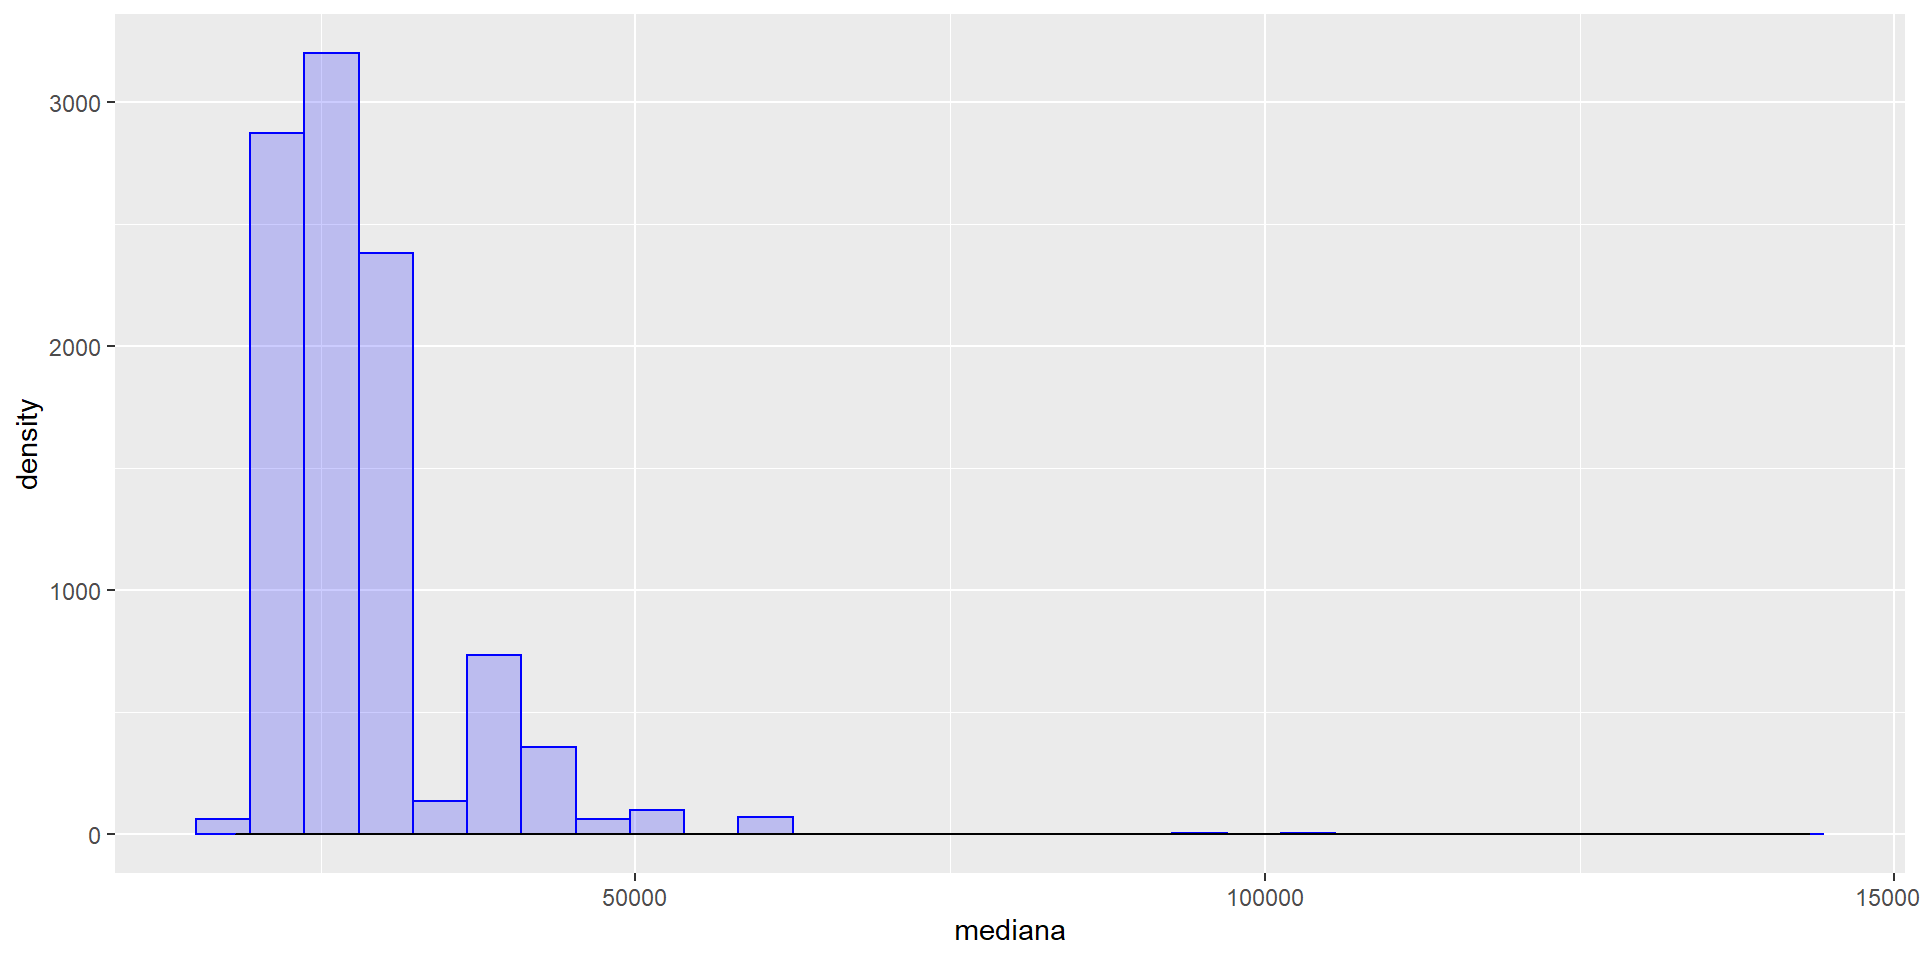
\includegraphics[width=0.7\textwidth]{Tema 3/figures/Figure 7}
\end{center}
\begin{tcolorbox}[colback=blue!5!white, colframe=blue!75!black, title=\textbf{Calculamos los percentiles 2.5\% y 97.5\%}]
\begin{lstlisting}
str_glue("El intervalo basado en percentiles Bootstrap para la mediana es: [{formatC(quantile(valores_medianas, 0.025), format = 'd')}, {formatC(quantile(valores_medianas, 0.975), format = 'd')}]")    
\end{lstlisting}
El intervalo basado en percentiles Bootstrap para la mediana es: [20654, 45720]
\end{tcolorbox}
\begin{tcolorbox}[colback=blue!5!white, colframe=blue!75!black, title=\textbf{Recordad que, con la aproximación $\hat{\theta}_n+1-96\cdot \hat{se}$,}]
    habíamos obtenido [14612,39235]
\end{tcolorbox}
\begin{lstlisting}
ingresos
\end{lstlisting}
\begin{verbatim}
## [1]  22010  43950  31416 143200  19298  21521  60025  24320  18221  29528
\end{verbatim}
\newpage
\documentclass{article}
\usepackage{fullpage}
\usepackage[utf8]{inputenc}
\usepackage{pict2e}
\usepackage{amsmath}
\usepackage{enumitem}
\usepackage{eurosym}
\usepackage{mathtools}
\usepackage{amssymb, amsfonts, latexsym, cancel}
\setlength{\parskip}{0.3cm}
\usepackage{graphicx}
\usepackage{fontenc}
\usepackage{slashbox}
\usepackage{setspace}
\usepackage{gensymb}
\usepackage{accents}
\usepackage{adjustbox}
\setstretch{1.35}
\usepackage{bold-extra}
\usepackage[document]{ragged2e}
\usepackage{subcaption}
\usepackage{tcolorbox}
\usepackage{xcolor, colortbl}
\usepackage{wrapfig}
\usepackage{empheq}
\usepackage{array}
\usepackage{parskip}
\usepackage{arydshln}
\graphicspath{ {images/} }
\renewcommand*\contentsname{\color{black}Índice} 
\usepackage{array, multirow, multicol}
\definecolor{lightblue}{HTML}{007AFF}
\usepackage{color}
\usepackage{etoolbox}
\usepackage{listings}
\usepackage{mdframed}
\setlength{\parindent}{0pt}
\usepackage{underscore}
\usepackage{hyperref}
\usepackage{tikz}
\usepackage{tikz-cd}
\usetikzlibrary{shapes, positioning, patterns}
\usepackage{tikz-qtree}
\usepackage{biblatex}
\usepackage{pdfpages}
\usepackage{pgfplots}
\usepackage{pgfkeys}
\addbibresource{biblatex-examples.bib}
\usepackage[a4paper, left=1cm, right=1cm, top=1cm,
bottom=1.5cm]{geometry}
\usepackage{titlesec}
\usepackage{titletoc}
\usepackage{tikz-3dplot}
\usepackage{kbordermatrix}
\usetikzlibrary{decorations.pathreplacing}
\newcommand{\Ej}{\textcolor{lightblue}{\underline{Ejemplo}}}
\setlength{\fboxrule}{1.5pt}

% Configura el formato de las secciones utilizando titlesec
\titleformat{\section}
{\color{red}\normalfont\LARGE\bfseries}
{Tema \thesection:}
{10 pt}
{}

% Ajusta el formato de las entradas de la tabla de contenidos
\addtocontents{toc}{\protect\setcounter{tocdepth}{4}}
\addtocontents{toc}{\color{black}}

\titleformat{\subsection}
{\normalfont\Large\bfseries\color{red}}{\thesubsection)}{1em}{\color{lightblue}}

\titleformat{\subsubsection}
{\normalfont\large\bfseries\color{red}}{\thesubsubsection)}{1em}{\color{lightblue}}

\newcommand{\bboxed}[1]{\fcolorbox{lightblue}{lightblue!10}{$#1$}}
\newcommand{\rboxed}[1]{\fcolorbox{red}{red!10}{$#1$}}

\DeclareMathOperator{\N}{\mathbb{N}}
\DeclareMathOperator{\Z}{\mathbb{Z}}
\DeclareMathOperator{\R}{\mathbb{R}}
\DeclareMathOperator{\Q}{\mathbb{Q}}
\DeclareMathOperator{\K}{\mathbb{K}}
\DeclareMathOperator{\im}{\imath}
\DeclareMathOperator{\jm}{\jmath}
\DeclareMathOperator{\col}{\mathrm{Col}}
\DeclareMathOperator{\fil}{\mathrm{Fil}}
\DeclareMathOperator{\rg}{\mathrm{rg}}
\DeclareMathOperator{\nuc}{\mathrm{nuc}}
\DeclareMathOperator{\dimf}{\mathrm{dimFil}}
\DeclareMathOperator{\dimc}{\mathrm{dimCol}}
\DeclareMathOperator{\dimn}{\mathrm{dimnuc}}
\DeclareMathOperator{\dimr}{\mathrm{dimrg}}
\DeclareMathOperator{\dom}{\mathrm{Dom}}
\DeclareMathOperator{\infi}{\int_{-\infty}^{+\infty}}
\newcommand{\dint}[2]{\int_{#1}^{#2}}

\newcommand{\bu}[1]{\textcolor{lightblue}{\underline{#1}}}
\newcommand{\lb}[1]{\textcolor{lightblue}{#1}}
\newcommand{\db}[1]{\textcolor{blue}{#1}}
\newcommand{\rc}[1]{\textcolor{red}{#1}}
\newcommand{\tr}{^\intercal}

\renewcommand{\CancelColor}{\color{lightblue}}

\newcommand{\dx}{\:\mathrm{d}x}
\newcommand{\dt}{\:\mathrm{d}t}
\newcommand{\dy}{\:\mathrm{d}y}
\newcommand{\dz}{\:\mathrm{d}z}
\newcommand{\dth}{\:\mathrm{d}\theta}
\newcommand{\dr}{\:\mathrm{d}\rho}
\newcommand{\du}{\:\mathrm{d}u}
\newcommand{\dv}{\:\mathrm{d}v}
\newcommand{\tozero}[1]{\cancelto{0}{#1}}
\newcommand{\lbb}[2]{\textcolor{lightblue}{\underbracket[1pt]{\textcolor{black}{#1}}_{#2}}}
\newcommand{\dbb}[2]{\textcolor{blue}{\underbracket[1pt]{\textcolor{black}{#1}}_{#2}}}
\newcommand{\rub}[2]{\textcolor{red}{\underbracket[1pt]{\textcolor{black}{#1}}_{#2}}}

\author{Francisco Javier Mercader Martínez}
\date{}
\title{Álgebra Lineal\\ Ejercicios Tema 3: Sistemas de ecuaciones y determinantes}
\renewcommand{\arraystretch}{1}
\setlength{\arraycolsep}{6pt}

\begin{document}
\maketitle
\begin{enumerate}[label=\color{red}\textbf{\arabic*)}]
    \item \lb{Sea $\{w_1,w_2,w_3\} $ un conjunto independiente de vectores de $\R^3$. Se definen los vectores $v_1=w_1+w_2,v_2=w_1+2w_2+w_3$ y $v_3=w_2+cw_3$. Si $V=[v_1,v_2,v_3]$ y $W=[w_1,w_2,w_3]$, entonces se tiene $V=WC$ con  \[
    C=\begin{bmatrix} 
        1 & 1 & 0\\
        1 & 2 & 1\\
        0 & 1 & c
    \end{bmatrix} 
    \]¿Qué condición debe cumplir $c$ para que los vectores  $v_1,v_2,v_3$ sean linealmente independientes? } 

    Para determinar la condición que debe cumplir $c$ para que los vectores  $v_1,v_2,v_3$ sean linealmente indpendientes, observa que:
\begin{enumerate}[label=\arabic*)]
\item \textbf{Los vectores $\{w_1,w_2,w_3\} $} son linealmente independientes en $\R^3$. Esto implica que la matriz \[
        W=[w_1,w_2,w_3]
    \] es invertible  (tiene determinante distinto de cero).
\item \textbf{Los vectores $\{v_1,v_2,v_3\} $} se pueden expresar como \[
        V=[v_1,v_2,v_3]=WC,
\] donde \[
C=\begin{bmatrix} 
    1 & 1 & 0 \\
    1 & 2 & 1\\
    0 & 1 & c
\end{bmatrix}. 
\] 
\item \textbf{Independencia lineal de $v_1,v_2,v_3$.} Puesto que $W$ es invertible  $v_1,v_2,v_3$ serán linealmente independientes si y solo si la matriz $C$ es invertible; es decir,  si y sólo si $\mathrm{det}(C)\neq 0$.
\item \textbf{Cálculo de $\mathrm{det}(C)$.} Calculamos el determinante de la matriz $C$:  \[
\mathrm{det}(C)=\begin{vmatrix} 
    1 & 1 & 0\\
    1 & 2 & 1\\
    0 & 1 & c
\end{vmatrix}=(2c+0+0)-(0+c+1)=2c-c-1=c-1 
\]  
\item \textbf{Condición de independencia.} Para que $C$ sea invertible, necesitamos  $\mathrm{det}(C)\neq 0$. Dado que \[
\mathrm{det}(C)=c-1,
\] se requiere \[
c-1\neq 0\longrightarrow c\neq 1.
\] 
\end{enumerate}
    \item \lb{Dadas las matrices \[
    A=\begin{bmatrix} 
        1 & 1 & -1\\
        2 & 4 & 2\\
        0 & 1 & 1\\
        3 & 2 & 1
    \end{bmatrix}\qquad B=\begin{bmatrix} 
        2 & 4 & 2\\
        3 & 2 & 1\\
        1 & 1 & -1\\
        0 & 1 & 1
    \end{bmatrix}  
    \]Halla una matriz de permutación $P$ tal que $PA=B$ y escribe  $P$ como producto de matrices de permutación simples.}

    Para encontrar una matriz de permutación $P$ tal que  $PA=B$, procedemos de la siguiente manera: 

     {
\renewcommand{\arraystretch}{1}
\setlength{\arraycolsep}{6pt}
$\begin{aligned}
      \left[ \begin{array}{ccc:cccc}
			1 & 1 & -1 & 1 & 0 & 0 & 0\\
			2 & 4 & 2 & 0 & 1 & 0 & 0\\
			0 & 1 & 1 & 0 & 0 & 1 & 0\\
			3 & 2 & 1 & 0 & 0 & 0 & 1
      \end{array} \right]& \xrightarrow{F_1\leftrightarrow F_2}      \left[ \begin{array}{ccc:cccc}
2 & 4 & 2 & 0 & 1 & 0 & 0\\
1 & 1 & -1 & 1 & 0 & 0 & 0\\
0 & 1 & 1 & 0 & 0 & 1 & 0\\
3 & 2 & 1 & 0 & 0 & 0 & 1
      \end{array} \right]\xrightarrow{F_3\leftrightarrow F_4}\left[ \begin{array}{ccc:cccc}
2 & 4 & 2 & 0 & 1 & 0 & 0\\
1 & 1 & -1 & 1 & 0 & 0 & 0\\
3 & 2 & 1 & 0 & 0 & 0 & 1\\
0 & 1 & 1 & 0 & 0 & 1 & 0
      \end{array} \right]\\
&\xrightarrow{F_2\leftrightarrow F_3}\left[ \begin{array}{ccc:cccc}
2 & 4 & 2 & 0 & 1 & 0 & 0\\
3 & 2 & 1 & 0 & 0 & 0 & 1\\
1 & 1 & -1 & 1 & 0 & 0 & 0 \\
0 & 1 & 1 & 0 & 0 & 1 & 0\\
      \end{array} \right]\Longrightarrow P=\begin{bmatrix}
0 & 1 & 0 & 0\\
0 & 0 & 0 & 1\\
1 & 0 & 0 & 0\\
0 & 0 & 1 & 0
\end{bmatrix}
     \end{aligned}$}
    \item \lb{Se tiene una matriz $A=(a_{ij})$ de tamaño $5\times 5$, donde $a_{ij}$ en la cantidad de mensajes que la persona $i$ manda a la persona $j$. Las filas y columnas siguen el orden: Juan, Ana, Pedro, María, Maite. Halla una matriz de permutación $P$ tal que las columnas y filas de  $PAP^\intercal$ sigan el orden: Ana, María, Juan, Maite, Pedro.}

        Para encontrar la matriz de permutación $P$ tal que las filas y columnas de  $PAP^\intercal$ estén en el orden deseado, seguimos estos paso:
        \begin{enumerate}[label=\arabic*)]
            \item Entender el problema:

                La matriz $A$ tiene filas y columas y columnas ordendas como: \[
                \text{Orden original: }\{\mathrm{Juan},\mathrm{Ana},\mathrm{Pedro}, \text{María},\text{Maite}\} .
                \] 
                Queremos reorganizar filas y columnas para que queden en este orden:
                \begin{center}
                    Nuevo orden: \{Ana, María, Juan, Maite, Pedro\}.
                \end{center}
                La matriz de permutación $P$ realizará este cambio
            \item Definir $P$:

                La matriz de permutación $P$ es una matriz identidad $5\times 5$ con las filas reordenadas de acuerdo con el nuevo orden. Cada fila de $P$ indica la nueva posición de una fila de la matriz identidad:
                \begin{itemize}[label=\textbullet]
                    \item El orden original:
                        \begin{itemize}[label=\textbullet]
                            \item Ana $(i=2)$ pasa a la posición 1.
                            \item María $(i=4)$ pasa a la posición 2.
                            \item Juan $(i=1)$ pasa a la posició 3.
                            \item Maite $(i=5)$ pasa a la posición 4.
                            \item Pedro $(i=3)$ pasa a la posición 5.
                        \end{itemize}
                \end{itemize}
                Entonces, $P$ se construye intercambiando las filas de la identidad en consecuencia: \[
                P=\begin{bmatrix} 
                    0 & 1 & 0 & 0 & 0\\
                    0 & 0 & 0 & 1 & 0\\
                    1 & 0 & 0 & 0 & 0\\
                    0 & 0 & 0 & 0 & 1\\
                    0 & 0 & 1 & 0 & 0
                \end{bmatrix} .
                \] 
            \item Interpretación de $PAP^\intercal$:

                La operación $PAP^\intercal$ realiza dos pasos:
                \begin{enumerate}[label=\arabic*)]
                    \item \textbf{Reorganizar las filas de $A$ según $P$}, es decir, poner las filas de $A$ en el orden especificado.
                    \item  \textbf{Reorganizar las columnas de $A$} (mediante $P^\intercal$) en el mismo orden.
                \end{enumerate}
        \end{enumerate}
    \item \lb{Consideremos la matriz por bloques $\begin{bmatrix} 
                A & B 
    \end{bmatrix} $ con $A$ una matriz de tamaño  $n\times n$ y $B$ una matriz de tamaño  $n\times p$. Supongamos que haciendo operaciones elementales de filas se obtiene la matriz $\begin{bmatrix} 
                I_n & X 
    \end{bmatrix} $. Prueba que $X=A^{-1}B$.}

    Para probar que $X=A^{-1}B$, analizamos el problema paso a paso:
    \begin{enumerate}[label=\arabic*)]
        \item Definición del problema.

            La matriz por bloques es \[
            \begin{bmatrix} 
                A & B 
            \end{bmatrix}, 
            \] donde $A$ es una matriz cuadrada de tamaño  $n\times n$, y $B$ es una matriz de tamaño  $n\times p$.

            Por hipótesis, haciendo operaciones elementales de filas, se transforma en \[
            \begin{bmatrix} 
                I_n & X 
            \end{bmatrix}, 
            \] donde $I_n$ es la matriz identidad de tamaño  $n\times n$ y $X$ es una matriz de tamaño  $n\times p$.

            Queremos demostrar que $X=A^{-1}B$.
        \item Operaciones elementales y equivalencia de filas:

            Hacer operaciones elementales de filas sobre una matriz equivale a multiplicarla a la izquierda por una matriz invertible $P$. Esto significa que existe una matriz  $P$ de tamaño $n\times n$ tal que: \[
            P\begin{bmatrix} 
                A & B 
            \end{bmatrix} =\begin{bmatrix} 
                I_n & X 
            \end{bmatrix} .
            \] 
            Separando los bloques, esta ecuación se escribe como: \[
            P\begin{bmatrix} 
            A & B 
            \end{bmatrix} =\begin{bmatrix} 
            PA & PB 
            \end{bmatrix} .
            \] 
            De la igualdad con $\begin{bmatrix} 
                I_n & X 
            \end{bmatrix} $, concluimos que: \[
            PA=I_n\quad \text{y}\quad PB=X.
            \] 
            De la igualda $PA=I_n$, vemos que  $P$ es la inversa de  $A$:  \[
            P=A^{-1}.
            \] 
            Sustituyendo $P=A^{-1}$ en $PB=X$, obtenemos:  \[
            X=A^{-1}B.
            \] 
    \end{enumerate}
    \item \lb{Halla una relación de dependencia entre los vectores $u_1=(1,0,1,0),\,u_2=(2,1,0,1),\,u_3=(0,2,-1,1)$ y $u_4=(3,-1,2,0)$.}

        Para encontrar una relación de dependencia lineal entre los vectores $u_1,u_2,u_3$ y $u_4$, necesitamos determinar si existen coeficientes $c_1,c_2,c_3,c_4$, no todos cero, tales que: \[
        c_1u_1+c_2u_2+c_3u_3+c_4u_4=0,
        \] o equivalentemente: \[
        c_1(1,0,1,0)+c_2(2,1,0,1)+c_3(0,2-1,1)+c_4(3,-1,2,0)=(0,0,0,0).
        \] 
        Esto genera el sistema de ecuaciones lineales: \[
        \begin{cases}
            c_1+2c_2+3c_4=0\\
            c_2+2c_3-c_4=0\\
            c_1-c_3+2c_4=0\\
            c_2+c_3=0
        \end{cases}
        \] 
        \begin{enumerate}[label=\arabic*)]
            \item Formar la matriz del sistema:

                Escribimos este sistema como una matriz aumentada: 
                \[
                    \begin{bmatrix}
                    1 & 2 & 0 & 3 & 0\\
                    0 & 1 & 2 & -1 & 0\\
                    1 & 0 & -1 & 2 & 0\\
                    0 & 1 & 1 & 0 & 0
                \end{bmatrix}
                \] 
            \item Resolver por eliminación gaussiana:

$\begin{aligned}\begin{bmatrix}
                    1 & 2 & 0 & 3 & 0\\
                    0 & 1 & 2 & -1 & 0\\
                    1 & 0 & -1 & 2 & 0\\
                    0 & 1 & 1 & 0 & 0
                \end{bmatrix}&\xrightarrow{F_3\to F_3-F_1}\begin{bmatrix}
                    1 & 2 & 0 & 3 & 0\\
                    0 & 1 & 2 & -1 & 0\\
                    0 & -2 & -1 & -1 & 0\\
                    0 & 1 & 1 & 0 & 0
                \end{bmatrix}\xrightarrow[F_4\to F_4-F_1]{F_3\to F_3+2F_1}\begin{bmatrix}
                    1 & 2 & 0 & 3 & 0\\
                    0 & 1 & 2 & -1 & 0\\
                    0 & 0 & 3 & -3 & 0\\
                    0 & 0 & -1 & 1 & 0
                \end{bmatrix}\\
&\xrightarrow{F_3\leftrightarrow F_4}\begin{bmatrix}
                    1 & 2 & 0 & 3 & 0\\
                    0 & 1 & 2 & -1 & 0\\
                    0 & 0 & -1 & 1 & 0\\
                    0 & 0 & 3 & -3 & 0\\
                \end{bmatrix}\xrightarrow{F_4\to F_4+3F_3}\begin{bmatrix}
                    1 & 2 & 0 & 3 & 0\\
                    0 & 1 & 2 & -1 & 0\\
                    0 & 0 & -1 & 1 & 0\\
                    0 & 0 & 0 & 0 & 0\\
                \end{bmatrix}\end{aligned}$

Esta matriz reducida resultante muestra que la última fila es cero, indicando una relación de dependencia lineal entre los vectores $u_1,u_2,u_3,u_4$.
\item Relación de dependencia:

    De la matriz reducida, obtenemos las ecuaciones: 
    \begin{itemize}[label=\textbullet]
        \item $c_1+c_4=0\longrightarrow c_1=-c_4$
        \item $c_2+c_4=0\longrightarrow c_2=-c_4$
        \item $c_3-c_4=0\longrightarrow c_3=c_4$
    \end{itemize}
    Al sustituir en la combinación lineal, podemos escribir la relación de dependencia como: \[
    c_1u_1+c_2u_2+c_3u_3+c_4u_4=0\quad \text{con}\quad c_1=c_2=-c_4,c_3=c_4.
    \] 
        \end{enumerate}
    \item \lb{Sean $A$ y  $B$ matrices del mismo tamaño. Sea  $A'$ la matriz que resulta de  $A$ después de intercambiar las columnas  $i,j$ y sea  $B'$ la matriz que resulta de  $B$ después de intercambiar las filas  $i,j$. Escribe las matrices  $A'$ y  $B'$ en términos de  $A,B$ y matrices elementales. ¿Por qué se verifica que $AB=A'B'$?}

        \begin{enumerate}[label=Paso \arabic*:]
            \item Representar $A'$ y  $B'$ en términos de matrices elementales

                Supongamos que  $A$ y  $B$ son matrices de tamaño  $n\times n$. Queremos describir las matrices $A'$ y  $B'$ que resultan al intercambiar columnas y filas, respectivamente.
                 \begin{enumerate}[label=1.\arabic*)]
                    \item Matriz $A'$:

                        Para obtener  $A'$, intercambiamos las columnas  $i$ y $j$ de $A$. Esto se logra multiplicando $A$ por una matriz de permutación  $P_{ij}$  desde la derecha: \[
                        A'=AP_{ij},
                        \] 
                        donde $P_{ij}$ es una matriz identidad $n\times n$ con las columnas $i$ y $j$ intercambiadas.
                    \item Matriz $B'$:

                        Para obtener  $B'$, intercambiamos las filas  $i$ y $j$ de $B$. Esto se logra multiplicando  $B$ por una matriz de permutación  $P_{ij}$  desde la izquierda: \[
                        B'=P_{ij}B.
                        \] 
                \end{enumerate}
            \item Producto $AB$ en términos de  $A'$ y $B'$  

                El producto $AB$ se transforma en $A'B'$. Sustituyendo  $A'=AP_{ij}$ y $B'=P_{ij}B$, tenemos: \[
                A'B'=(AP_{ij})(P_{ij}B).
                \] 
                Por la propiedad asociativa del producto de matrices: \[
                    A'B'=A(P_{ij}P_{ij})B.
                \] 
                La clave es que $P_{ij}$ es una matriz de permutación, y el producto de una matriz de permutación consigo misma es la identidad: \[
                P_{ij}P_{ij}=I.
                \] 
                Por lo tanto: \[
                A'B'=AIB=AB.
                \] 
        \end{enumerate}
    \item \lb{Calcula el rango de la matriz \[
    B=\begin{bmatrix} 
        a & 0 & 0 & b\\
        b & a & 0 & 0\\
        0 & b & a & 0\\
        0 & 0 & b & a
    \end{bmatrix} 
    \]en función de los parámetros $a$ y  $b$.}

    \underline{Posibles casos:}
    \begin{enumerate}[label=\arabic*)]
        \item $a=b=0\longrightarrow B=[0]\longrightarrow \mathrm{rango}(B)=0$ 
        \item $a=0,b\neq 0\longrightarrow B=\begin{bmatrix} 
                0 & 0 & 0 & b\\
                b & 0 & 0 & 0\\
                0 & b & 0 & 0\\
                0 & 0 & b & 0
                \end{bmatrix}\xrightarrow{C_4\to C_1}\underset{\text{forma escalonada}}{\begin{bmatrix} 
                b & 0 & 0 & 0\\
                0 & b & 0 & 0\\
                0 & 0 & b & 0\\
                0 & 0 & 0 & b
        \end{bmatrix}}\longrightarrow \mathrm{rango}(B)=4  $ 
        \item $a\neq 0,b=0\longrightarrow B=\begin{bmatrix} 
                a & 0 & 0 & 0\\
                0 & a & 0 & 0\\
                0 & 0 & a & 0\\
                0 & 0 & 0 & a
        \end{bmatrix}\longrightarrow \mathrm{rango}(B)=4 $
    \end{enumerate}

    \item \lb{Dada la matriz $M=\begin{bmatrix} 
                2 & 0 & 2 & 6\\
                1 & 1 & 0 & 2\\
                3 & 2 & 1 & 7
    \end{bmatrix} $ calcula matrices invertibles $P$ y  $Q$ tales que  \[
    PMQ=\left[ \begin{array}{c|c}
            1_r & 0\\ \hline
            0 & 0
    \end{array} \right] 
    \] con $r$ el rango de $M$.}

$\begin{aligned}
\left[ 
    \begin{array}{cccc|ccc}
        2 & 0 & 2 & 6 & 1 & 0 & 0\\
        1 & 1 & 0 & 2 & 0 & 1 & 0\\
        3 & 2 & 1 & 7 & 0 & 0 & 1
    \end{array}
    \right]& \xrightarrow{F_1\leftrightarrow F_2}\left[ \begin{array}{cccc|ccc}
            1 & 1 & 0 & 2 & 0 & 1 & 0\\
            2 & 0 & 2 & 6 & 1 & 0 & 0\\
            3 & 2 & 1 & 7 & 0 & 0 & 1
    \end{array} \right] \xrightarrow[F_3\to F_3-3F_1]{F_2\to F_2-2F_1} \left[ \begin{array}{cccc|ccc}
            1 & 1 & 0 & 2 & 0 & 1 & 0\\
            0 & -2 & 2 & 2 & 1 & -2 & 0\\
            0 & -1 & 1 & 1 & 0 & -3 & 1\\
    \end{array} \right]\\
           & \xrightarrow{F_2\leftrightarrow F_3}\left[ \begin{array}{cccc|ccc}
            1 & 1 & 0 & 2 & 0 & 1 & 0\\
            0 & -1 & 1 & 1 & 0 & -3 & 1 \\
            0 & -2 & 2 & 2 & 1 & -2 & 0
    \end{array} \right] \xrightarrow{F_3\to F_3-2F_2}\left[ \begin{array}{cccc|ccc}
            1 & 1 & 0 & 2 & 0 & 1 & 0\\
            0 & -1 & 1 & 1 & 0 & -3 & 4\\
            0 & 0 & 0 & 0 & 1 & 4 & -2
    \end{array} \right]\\
           & \xrightarrow{F_2\to -F_2}\left[ \begin{array}{cccc|ccc}
            1 & 1 & 0 & 2 & 0 & 1 & 0\\
            0 & 1 & -1 & -1 & 0 & 3 & 1\\
            0 & 0 & 0 & 0 & 1 & 4 & -2
    \end{array} \right] \longrightarrow P=\begin{bmatrix} 
            0 & 1 & 0\\
            0 & 3 & -1\\
            1 & 4 & -2
    \end{bmatrix} 
\end{aligned}$

$\begin{aligned}\left[\begin{array}{cccc}
    1 & 1 & 0 & 2\\ 
    0 & 1 & -1 & -1\\
    0 & 0 & 0 & 0\\ \hline
    1 & 0 & 0 & 0\\
    0 & 1 & 0 & 0\\
    0 & 0 & 1 & 0\\
    0 & 0 & 0 & 1
\end{array}\right]&\xrightarrow[C_4\to C_4-2C_1]{C_2\to C_2-C_1}\left[ \begin{array}{cccc}
    1 & 0 & 0 & 0\\
    0 & 1 & -1 & -1\\
    0 & 0 & 0 & 0\\ \hline
    1 & -1 & 0 & -2\\
    0 & 1 & 0 & 0\\
    0 & 0 & 1 & 0\\
    0 & 0 & 0 & 1
\end{array} \right] \xrightarrow[C_4\to C_4-C_2]{C_{3}\to C_3-C_2}\left[ \begin{array}{cccc}
    1 & 0 & 0 & 0\\
    0 & 1 & 0 & 0\\
    0 & 0 & 0 & 0\\ \hline
    1 & -1 & 1 & -1\\
    0 & 1 & -1 & -1\\
    0 & 0 & 1 & 0\\
    0 & 0 & 0 & 1
\end{array} \right]\\ 
& \longrightarrow Q=\begin{bmatrix} 
    1 & -1 & 1 & -1\\
    0 & 1 & -1 & -1\\
    0 & 0 & 1 & 0\\
    0 & 0 & 0 & 1
\end{bmatrix}\end{aligned}$

Finalmente tenemos una matriz $PMQ=\begin{bmatrix} 
    1 & 0 & 0 & 0\\
    0 & 1 & 0 & 0\\
    0 & 0 & 0 & 0
\end{bmatrix} $ que tiene la forma \[
\left[ \begin{array}{c|c}
        I_n & 0\\ \hline
        0 & 0
\end{array} \right] 
\] donde $I_r$ es la matriz identidad con  $r=\mathrm{rango}(M)=2$.

    \item \lb{Halla la inversa de la matriz $A=\begin{bmatrix} 
                1 & 1 & -3\\
                3 & 4 & -2\\
                -1 & -1 & 2
    \end{bmatrix} $ y expresa $A$ y  $A^{-1}$ como producto de matrices elementales.} 


\item \lb{Determina el valor del parámetro $a$ para el cual la matriz $A=\begin{bmatrix} 
            1 & 0 & 0 & 0\\
            a & 1 & 0 & 0\\
            a^2 & a & 1 & 0\\
            a^3 & a^2 & a & 1
\end{bmatrix} $ es invertible y calcula su inversa} 

\item \lb{Resuelve el siguiente sistema de ecuaciones lineales \[
\left.\begin{array}{r}
    x+2y-z-2t=5\\
    -2x-4y+2z+4t=-10\\
    y+t=1\\
    x+3y-z-t=6\\
    x-z-4t=3
\end{array}\right\}
\] } 

\item \lb{Discute en el cuerpo de los números reales los siguientes sistemas de ecuaciones en función del parámetro $a$  \[
\left\{ \begin{array}{rcrcrcrcc}
        x & + & ay & & & + & at & = & a\\
        ax & + & y & + & z & + & t & = & a\\
        x & + & y & az & + & t & = & 1
\end{array} \right. 
\] } 

\item \lb{Si $A=[u_1,\dots,u_n]$, expresa el determinante de $B=[u_n u_1\cdots u_{n-1}]$ en función del determinante de $A$.}

\item \lb{Una matriz $A$ que cumple  $A=-A^\intercal$ se llama \textbf{antisimétrica}. Prueba que una matriz antisimétrica e tamaño impar tiene determinante nulo. }

\item \lb{Calcula el determinante \[
\begin{vmatrix} 
    1 & 2 & 3 & \cdots & n\\
    2 & 3 & 4 & \cdots & n+1\\
    \vdots & \vdots & \vdots & & \vdots\\
    n & n+1 & n+2 & \cdots & 2n-1
\end{vmatrix} 
\] } 

\item \lb{
\setlength{\arraycolsep}{1pt}
Considera el sistema de ecuaciones \[
\left.\begin{array}{rl}
2x+y+z&=0\\
4x-6y-2x&=2\\
-2x+15y+7z&=-4
\end{array}\right\}
\]
Observa que podemos eliminar la última ecuación pues es combinación lineal de las dos primeras. Considerando ahora los términos en $z$ como si fuesen términos independientes, observa que el sistema es un sistema de Cramer en  $x,y$.  Resuélvelo con la fórmula de Cramer y después expresa las soluciones en la forma $x_0+u$ ($x_0$ solución parcial y $u$ solución genérica del sistema homogéneo).} 
\end{enumerate}
\end{document}

